%%%%%%%%%%%%%%%%%%%%%%%%%%%%%%%%%%%%%%%%%
% Wenneker Assignment
% LaTeX Template
% Version 2.0 (12/1/2019)
%
% This template originates from:
% http://www.LaTeXTemplates.com
%
% Authors:
% Vel (vel@LaTeXTemplates.com)
% Frits Wenneker
%
% License:
% CC BY-NC-SA 3.0 (http://creativecommons.org/licenses/by-nc-sa/3.0/)
% 
%%%%%%%%%%%%%%%%%%%%%%%%%%%%%%%%%%%%%%%%%

%----------------------------------------------------------------------------------------
%	PACKAGES AND OTHER DOCUMENT CONFIGURATIONS
%----------------------------------------------------------------------------------------

\documentclass[11pt]{scrartcl} % Font size
\usepackage{comment}
\usepackage{color}
%%%%%%%%%%%%%%%%%%%%%%%%%%%%%%%%%%%%%%%%%
% Wenneker Assignment
% Structure Specification File
% Version 2.0 (12/1/2019)
%
% This template originates from:
% http://www.LaTeXTemplates.com
%
% Authors:
% Vel (vel@LaTeXTemplates.com)
% Frits Wenneker
%
% License:
% CC BY-NC-SA 3.0 (http://creativecommons.org/licenses/by-nc-sa/3.0/)
% 
%%%%%%%%%%%%%%%%%%%%%%%%%%%%%%%%%%%%%%%%%

%----------------------------------------------------------------------------------------
%	PACKAGES AND OTHER DOCUMENT CONFIGURATIONS
%----------------------------------------------------------------------------------------

\usepackage{amsmath, amsfonts, amsthm} % Math packages
\usepackage{tabto}
\usepackage{listings} % Code listings, with syntax highlighting
\usepackage{tabu}
\usepackage{array}
\usepackage[english]{babel} % English language hyphenation
\usepackage{hyperref}

\usepackage{graphicx} % Required for inserting images
\graphicspath{{Figures/}{./}} % Specifies where to look for included images (trailing slash required)

\usepackage{booktabs} % Required for better horizontal rules in tables

\numberwithin{equation}{section} % Number equations within sections (i.e. 1.1, 1.2, 2.1, 2.2 instead of 1, 2, 3, 4)
\numberwithin{figure}{section} % Number figures within sections (i.e. 1.1, 1.2, 2.1, 2.2 instead of 1, 2, 3, 4)
\numberwithin{table}{section} % Number tables within sections (i.e. 1.1, 1.2, 2.1, 2.2 instead of 1, 2, 3, 4)

\setlength\parindent{0pt} % Removes all indentation from paragraphs

\usepackage{enumitem} % Required for list customisation
\setlist{noitemsep} % No spacing between list items

%----------------------------------------------------------------------------------------
%	DOCUMENT MARGINS
%----------------------------------------------------------------------------------------

\usepackage{geometry} % Required for adjusting page dimensions and margins

\geometry{
	paper=a4paper, % Paper size, change to letterpaper for US letter size
	top=2.5cm, % Top margin
	bottom=3cm, % Bottom margin
	left=3cm, % Left margin
	right=3cm, % Right margin
	headheight=0.75cm, % Header height
	footskip=1.5cm, % Space from the bottom margin to the baseline of the footer
	headsep=0.75cm, % Space from the top margin to the baseline of the header
	%showframe, % Uncomment to show how the type block is set on the page
}

%----------------------------------------------------------------------------------------
%	FONTS
%----------------------------------------------------------------------------------------

\usepackage[utf8]{inputenc} % Required for inputting international characters
\usepackage[T1]{fontenc} % Use 8-bit encoding

\usepackage{fourier} % Use the Adobe Utopia font for the document

%----------------------------------------------------------------------------------------
%	SECTION TITLES
%----------------------------------------------------------------------------------------

\usepackage{sectsty} % Allows customising section commands

\sectionfont{\vspace{6pt}\centering\normalfont\scshape} % \section{} styling
\subsectionfont{\normalfont\bfseries} % \subsection{} styling
\subsubsectionfont{\normalfont\itshape} % \subsubsection{} styling
\paragraphfont{\normalfont\scshape} % \paragraph{} styling

%----------------------------------------------------------------------------------------
%	HEADERS AND FOOTERS
%----------------------------------------------------------------------------------------

\usepackage{scrlayer-scrpage} % Required for customising headers and footers

\ohead*{} % Right header
\ihead*{} % Left header
\chead*{} % Centre header

\ofoot*{} % Right footer
\ifoot*{} % Left footer
\cfoot*{\pagemark} % Centre footer
 % Include the file specifying the document structure and custom commands
\usepackage{graphicx}
\usepackage{subcaption}



%Code retrieved from: https://www.overleaf.com/project/5c52d66b6343590b46b4fd03


%----------------------------------------------------------------------------------------
%	TITLE SECTION
%----------------------------------------------------------------------------------------

\title{	
	\normalfont\normalsize
	\textsc{Old Dominion University}\\ % Your university, school and/or department name(s)
	\vspace{25pt} % Whitespace
	\rule{\linewidth}{0.5pt}\\ % Thin top horizontal rule
	\vspace{20pt} % Whitespace
	{\huge Assignment 2}\\ % The assignment title
	\vspace{12pt} % Whitespace
	\rule{\linewidth}{2pt}\\ % Thick bottom horizontal rule
	\vspace{12pt} % Whitespace
}

\author{\LARGE David Bayard} % Your name

\date{\normalsize\today} % Today's date (\today) or a custom date

\begin{document}

\definecolor{codegreen}{rgb}{0,0.6,0}
\definecolor{codegray}{rgb}{0.5,0.5,0.5}
\definecolor{codepurple}{rgb}{0.58,0,0.82}
\definecolor{backcolour}{rgb}{0.95,0.95,0.92}
\lstdefinestyle{pythonStyle}{
  backgroundcolor=\color{backcolour},  
  commentstyle=\color{codegreen},
  keywordstyle=\color{magenta},
  numberstyle=\tiny\color{codegray},
  stringstyle=\color{codepurple},
  basicstyle=\footnotesize,
  breakatwhitespace=false,         
  breaklines=true,                 
  captionpos=b,                    
  keepspaces=true,                 
  numbers=left,                    
  numbersep=5pt,                  
  showspaces=false,                
  showstringspaces=false,
  showtabs=false,                  
  tabsize=2
}

\lstset{style=pythonStyle}


\maketitle % Print the title

%----------------------------------------------------------------------------------------
%	FIGURE EXAMPLE
%----------------------------------------------------------------------------------------
\pagebreak
\section*{Question 1.}

%\begin{figure}[h] % [h] forces the figure to be output where it is defined in the code (it suppresses floating)
	%\centering
	%\includegraphics[width=0.5\columnwidth]{swallow.jpg} % Example image
	%\caption{European swallow.}
%\end{figure}

%------------------------------------------------

\subsection*{Write a Python program that extracts 1000 unique 
(collect more e.g., 1300 just in case) links from
Twitter. Omit links from the Twitter domain (twitter.com). Also note that you need to verify that the final target URI (i.e.,
the one that responds with a 200) is unique.} 
\bigskip\bigskip


\LARGE Solution:
\newline \newline\small

\tabto{2.0cm} The Twitter API offers users the ability to extract tweets from Twitter, by automating GET requests and responding with Tweet objects. Using this API resulted in JSON formatted Tweets, which could then be scanned for URIs.\newline

\tabto{2.0cm} Although, target links were only available for the past 7 days using this API, thus popular queries were used including ``Sports'', ``Trump'', ``Republicans'', and ``Immigration''. The snippet of code listed below displays the Search method from the Tweepy API. 

\begin{lstlisting}[language = Python, caption=Tweepy API Search Method]
for tweet in tweepy.Cursor(api.search, q="Immigration -filter:retweets",count = tweetsCountMax, include_entities=True).items(maxNumTweets):
\end{lstlisting} \bigskip \bigskip

\tabto{2.0cm} Once the Tweets have been gathered, the URI's are extracted by accessing the ``expanded url'' attribute of all the Tweet objects. The collected URI's are filtered for uniqueness by deduplicating and extending the URI's. Issues were encountered in this portion of the assignment, where shortened links were not completely extended. The code below implements a loop which will call ``filterLinksFunc(link)'', which will follow redirections and return a URI and status code. A counter was implement to prevent an infinite loop from occurring.

\begin{lstlisting}[language = Python, caption=Extending URI's]
    try:
      link, statusCode = filterLinksFunc(URL)

      if(statusCode == 200):
        newList.append(link)

      else:
        counter = 0;
        while(statusCode != 200 and counter != 5):
          filterLinksFunc(link)
          counter = counter + 1

    except:
      genericErrorInfo()
\end{lstlisting} \bigskip \bigskip
\pagebreak
\tabto{2.0cm} After extending all of the URI's, a deduplication function was applied to remove duplicate functions and guarantee uniqueness. This was accomplished by breaking each URI into its seperate components and comparing it to other existing URI's. Using this same concept, the domain names of   ``Twitter.com'' were removed.

\begin{lstlisting}[language = Python, caption=Deduplicating URI's]
    for URI in unsanitizedList:
      scheme, netloc, path, params, query, fragment = urlparse(URI)
      toCheck = netloc + path

    
      if toCheck not in deduplicatedList:
          deduplicatedList.append(URI)
  except:
    genericErrorInfo()

  return set(deduplicatedList)
\end{lstlisting} \bigskip \bigskip

\pagebreak

\section*{Question 2}\bigskip


\subsection*{Download the TimeMaps for each of the target URIs.  We'll use the ODU 
Memento Aggregator}

%------------------------------------------------
\bigskip\bigskip
\Large Solution: \newline\newline\small

\tabto{2.0cm} In order to download the TimeMaps for each target URI, Docker was installed and the MemGator image was downloaded. This allowed requests to be made via the local machine, rather than making requests through the ODU server. As stated above, the TimeMaps were downloaded by making GET requests via the localhost, which were sent to port 1208 of the server. The specific command used: sudo docker continer run --rm -it -p 5000:1208 ibnesayeed/memgator server

\begin{lstlisting}[language = Python, caption=Make TimeMap Request]
##### Make Request and store the JSON response in json_obj
      
      requestToMake = "http://localhost:5000/timemap/json/" + URI

      resp = requests.get(requestToMake, timeout=30)

      ##Write response in json format ##
      json_obj = resp.json()
\end{lstlisting} 

\tabto{2.0cm}Once a JSON object is created from the request, it is possible to read the response, and parse the data as shown.

\begin{lstlisting}[language = Python, caption=JSON Request]
##### Make Request and store the JSON response in json_obj
      dataGood = {"URI" : "value", "Mementos" : "value2", "TimeMapFileName" : "value3" }

      dataGood["URI"] = URI
        dataGood["Mementos"] = len(json_obj["mementos"]["list"])
        dataGood["TimeMapFileName"] = fileName
\end{lstlisting} 

\tabto{2.0cm}The code above displays that the JSON format provides access to the content of the response, which is parsed earlier using the ``resp.json()'' function. This methodology is used through the entire program, making it simple to store and retrieve data from files, simplifying the program. Moreover, after extracting the JSON data, it is convenient to append the data to a dictionary, and create a list of dictionaries. Then, this list of dictionaries can be written to a .json file, and can easily be accessed later in the program.

\begin{lstlisting}[language = Python, caption=Writing JSON to file]
allMementosText.write("URI: " + dataGood["URI"])
        allMementosText.write("\n")
        allMementosText.write("TimeMapFileName: " + dataGood["TimeMapFileName"])
        allMementosText.write("\n")
        allMementosText.write("Mementos: " + str(dataGood["Mementos"]))
        allMementosText.write("\n\n\n")

        #allMementos is file being written to
        json.dump(dataGood, allMementos, indent=2)

        list.append(len(json_obj["mementos"]["list"]))
        print("Added " + str(len(json_obj["mementos"]["list"])))
\end{lstlisting} 

\begin{figure}[h!]
\begin{subfigure}[b]{0.9\linewidth }
    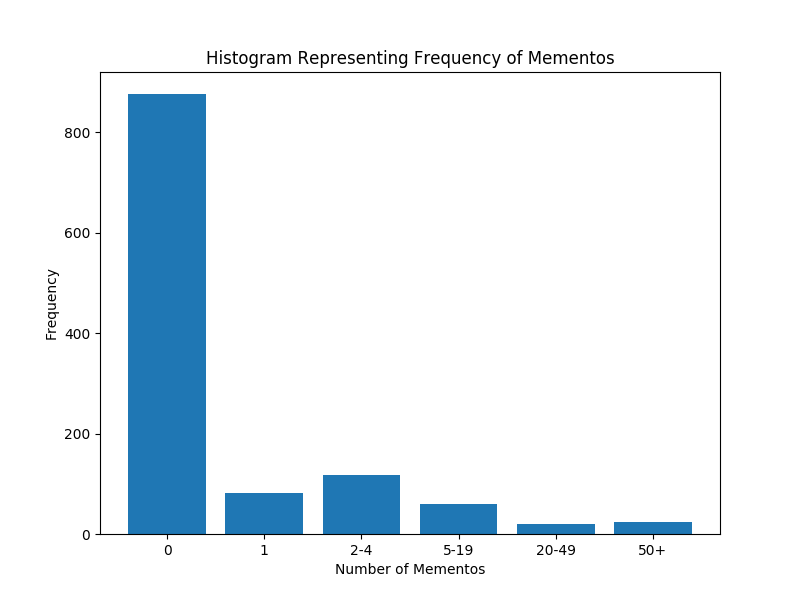
\includegraphics[width=\linewidth]{MementoVsURI.png}
    \caption{Histogram representing URI vs Number of Mementos}
\end{subfigure}
\end{figure}

\pagebreak
\section*{Question 3} \bigskip 

\subsection*{Estimate the age of each of the 1000 URIs using the "Carbon
Date" tool:}

\tabto{2.0cm}The exact same methodology from question 2 can be applied here to get the estimated age of each URI. This is achieved by launching the Docker container for the ``Carbon Date tool'' using the command ``sudo docker container run --rm -it -p 8888:8888 oduwsd1/carbonate -s''.\newline With the Carbonate container running, each request is processed through Carbonate, and every response is stored within the ``CarbonRecords.json'' file.

\begin{lstlisting}[language = Python, caption=Make Carbon Date Request]

  for URI in listURI:

    try:

      requestToMake = "http://localhost:8888/cd/" + URI
      resp = requests.get(requestToMake)



    except:
      genericErrorInfo()

    try:
      json_obj = resp.json()

    except:
      genericErrorInfo()
\end{lstlisting} \bigskip \bigskip
 
 \tabto{2.0cm} Using the ``CarbonRecords.json'' and ``MementosTrack.json'' files, a scatter plot is created representing the number of Mementos, and the estimated creation date of the URI corresponding to the URI.
 

 \begin{lstlisting}[language = Python, caption= Number of Mementos vs Age in days]
    for link in URIBoth:
  for a in carbontoData:
    if(a["URI"] == link and a["Carbon-Date"] != ""):
      
      toParse = a["Carbon-Date"]
      carbonDate = dateutil.parser.parse(toParse).date()

      age =  abs((today - carbonDate).days)


      ageVsMemento["Age"] = age

      
      for b in mementoData:
        if(b["URI"] == link):
          ageVsMemento["MementoCount"] = int(b["Mementos"])
          ageVsMementoList.append(ageVsMemento.copy())
\end{lstlisting} \bigskip \bigskip

\tabto{2.0cm} The main function of the code above is to parse the date from each URI that has a Carbon-Date, as well as the number of Mementos corresponding to the URI. This method is not efficient, but the design of the program prevented a more efficient approach. In the future, a preferred course would be to write all of the data to a single JSON file, making the process of parsing simple. Regardless, the data was gathered and the results were used to create the scatter plot depicted below.

\begin{figure}[h!]
\begin{subfigure}[b]{0.9\linewidth }
    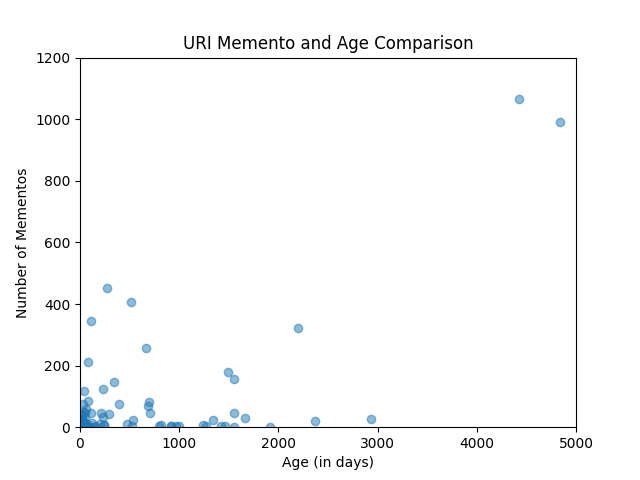
\includegraphics[width=\linewidth]{DatesVsMementos.png}
    \caption{Scatter Plot of Memento Count vs Age of URI}
\end{subfigure}
\end{figure}

In total, the results for the URIs, creation dates, and number of Mementos is categorized as shown below: \newline \newline
Total URIs: 1179 \newline
Number of URIs with Mementos: 303\newline
Number of URIs with Estimated Creation Dates:1017\newline

This information states that out of 1179 URIs, 1017 of them had estimated creation dates, and only 303 of them has at least one Memento.



\end{document}
